\documentclass[a4paper]{article}

\def\doctitle{实验三十四\ 全息照相}

\def\docabstract{全息照相(Holography)是能够把来自物体的光波波阵面的振幅和相位的信息记录下来,又能在需要时再现出这种光波的一种技术。这次实验将体验全息片的制作,并尝试用其再现出像。}

\def\dockeywords{全息术}

\usepackage{see-exp}

\def\doctoc{false}

\begin{document}

%title
\input{/home/supercgor/texmf/exp-titlepage.tex}

%contents here
\section{实验概要}
\subsection{实验目的}
\begin{enumerate}
    \item 了解全息照相的基本原理;
    \item 学习全息照相的实验技术,拍摄合格的全息图;
    \item 了解摄影暗室技术。
\end{enumerate}
\subsection{实验仪器}
\begin{enumerate}
    \item 光学平台、扩束透镜、反射镜和分束器、被摄物;
    \item 氦氖激光器及电源、快门;
    \item 暗室技术使用的设备。
\end{enumerate}

\subsection{实验原理}
\hspace{2em}在全息照相中,总共有两列波发生干涉:参考光与物体表面反射的光。对于参考光,可以选择平行光或球面光。在本次实验中,我们使用的是发散球面光作为参考光。\par
\hspace{2em} 在实验中获得的屏函数可以表现为一下线性形式:
\begin{align*}
    t_H & =t_0+\beta I_H, I_H=(O+R)(O^\star+R^\star)                 \\
    t_H & =t_0+\beta (|O|^2+|R|^2)+\beta R O^\star + \beta R^\star O
\end{align*}
其中$R$是参考光波前,$O$是物光波前。\par
\hspace{2em} 可以看到,在再现时会有三束透射光,三束透射光的屏函数分别记为:
\begin{equation*}
    \begin{cases}
        T_1 & =t_0+\beta(|O|^2+|R|^2) \\
        T_2 & =\beta R^\star O        \\
        T_3 & =\beta R O^\star
    \end{cases}
\end{equation*}\par
\hspace{2em} 在实验中,$T_1$代表的是衍射光的背景光,在实验中通常表现为比较微弱的散射光,所以在处理是会把它忽略掉。利用不同的再现光照射,可以得到不同的光学变换与不同性质的再现像。 \par

\section{实验记录}
\subsection{再现光路}
\hspace{2em} 在本次实验,物体光程为$\SI{97}{\cm}$,参考光程为$\SI{100}{\cm}$。两者差距约为$\SI{3}{\cm}$,曝光时间为$\SI{3.5}{\s}$。光路如图\ref{fig:1}所示。
\par
\begin{figure}[H]
    \centering
    %%%%%%%%%%%%%%%%%%%%%%%%%%%%%
    \begin{subfigure}[t]{0.4\textwidth}
        \centering
        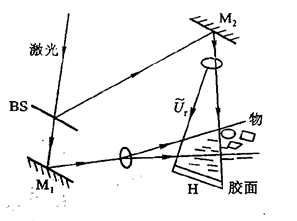
\includegraphics[width=\textwidth]{fig1.png}
        \captionsetup{font={normalsize,sf},justification=centering}
        \caption{}
        \label{fig:1}
    \end{subfigure}
    \begin{subfigure}[t]{0.4\textwidth}
        \centering
        \includegraphics[width=\textwidth]{fig3.jpg}
        \captionsetup{font={normalsize,sf},justification=centering}
        \caption{}
        \label{fig:2}
    \end{subfigure}
    %%%%%%%%%%%%%%%%%%%%%%%%%%%%%
    \captionsetup{justification=centering,subrefformat=parens}
    \caption{记录光路\subref{fig:1}示意图;\subref{fig:2}实际图。}
\end{figure}

\begin{figure}[H]
    \centering
    \captionsetup{justification=centering,margin=2cm}
    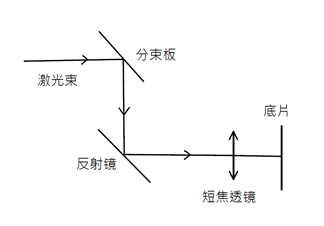
\includegraphics[width=.4\textwidth]{fig2.png}
    \caption{再现光路示意图}
\end{figure}

\subsection{原位观察虚像}
\begin{enumerate}
    \item 像处于原物的位置,大小与原物等大,是正立虚像。
          \\\textbf{分析}:由于再现光就是当时的参考光,参考光与再现光之间的相位被消掉,所以把当时记录的物光完整的复现出来,但由于有$\beta$的作用,光强会发生改变。
    \item 从底片不同的角度位置观察,像的性质、大小与位置均不发生改变。
          \\\textbf{分析}:由于只是把当时记录的物光完整的复现出来,没有相位的作用,只有光强的变化。
    \item 旋转底片,改变入射角,可以看到像发生了偏离。
          \\\textbf{分析}:这个时候再现光与参考光之间有了一个固定的相位差,形式为$e^{ik\varphi}$,作用等效于一个薄棱镜。所以看到的效果相当于像有了一个偏离。
    \item 改变底片与光源之间的距离,当距离变大时,像的横向放大率变大;当距离变小时,像的横向放大率变小。
          \\\textbf{分析}:可以近似认为是傍轴球面波,参考光与再现光两个二次相因子,等效成$\frac{1}{f}=\frac{1}{z}-\frac{1}{z^\prime}$,也就是一个透镜。其中z是光源与底片之间的距离,$z^\prime$是虚像与底片的距离,f是底片的等效焦距。当z增大时,$z^\prime$也会增大,在保持成虚像的前提下,物的横向放大率会变大。反之亦然。
\end{enumerate}

\begin{figure}[H]
    \centering
    \captionsetup{justification=centering,margin=2cm}
    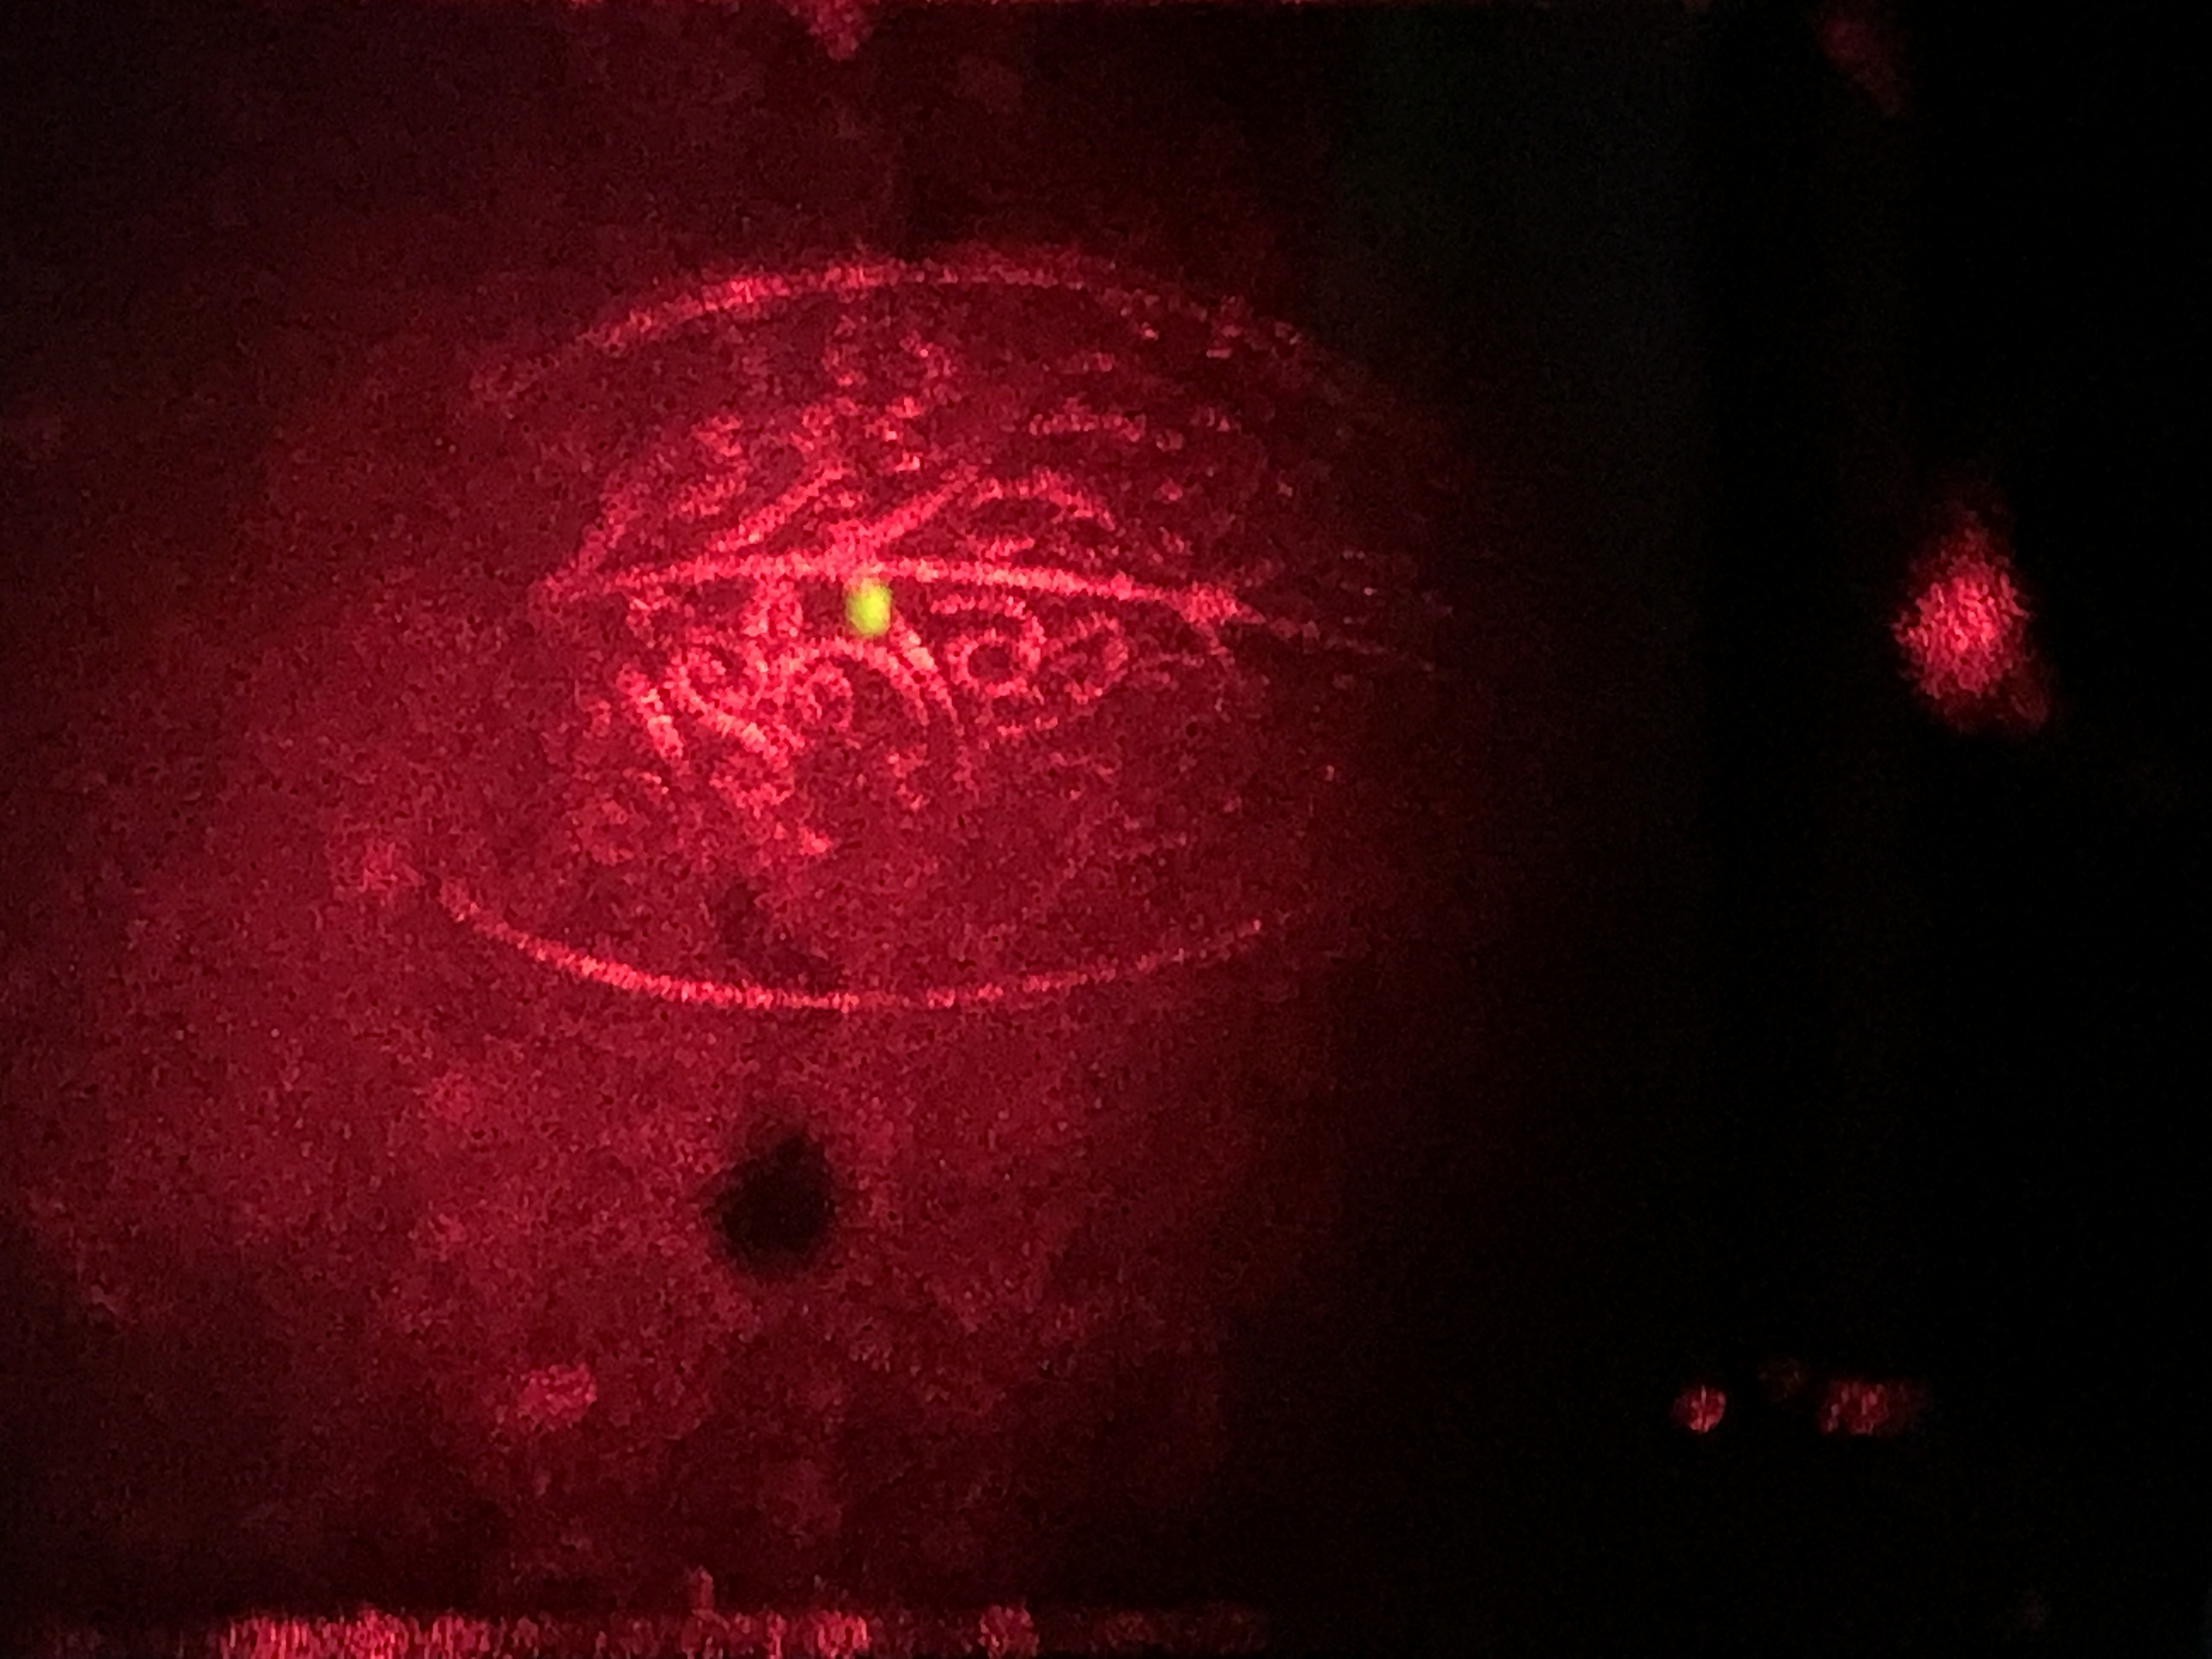
\includegraphics[width=.4\textwidth]{fig4.jpg}
    \caption{原位再现的像}
\end{figure}
\subsection{观察-1级衍射像}
\hspace{2em} 在上一个实验中,我们观察到的是$+1$级的衍射像,其代表的屏函数是。 \par
$$T_2=\beta R^\ast O$$
\hspace{2em} 对于-1级衍射像,代表的屏函数是 \par
$$T_3=\beta RO^\ast$$
\hspace{2em} 其中$O^\ast$代表的是物光的共轭光,由于在本次实验中使用的参考光是一个球面光,所以所成的像可以是实像或虚像。但这个是有前提的,就是底板的乳胶层是无限薄的,也就是说参考光与物光之间的夹角很小。但当夹角比较大的时候,比如在本次实验中夹角约为30°,乳胶层的厚度就已经不能忽略了。在本次实验中全息图是具有立体结构,相当于一个布拉格衍射。这个导致了只有在一定角度,也就是满足布拉格方程是,才会有比较明亮的重现像,同时使得$\pm1$级的像不会同时出现,因为在观察到-1级衍射像的前提下,+1级的衍射像方向不满足布拉格方程。在本次实验中,并没有观察到+1级衍射像。 \par

\subsection{底片反转180°,利用共轭光观察}
\hspace{2em} 可以观察到1个实像,但其位置十分之难找出。 原因可能是因为在记录时物光的散射太弱了,导致在使用会聚球面波重现时实像比较弱,需要在特别的位置进行阻挡才出现较好看的实像。\par
\begin{figure}[H]
    \centering
    \captionsetup{justification=centering,margin=2cm}
    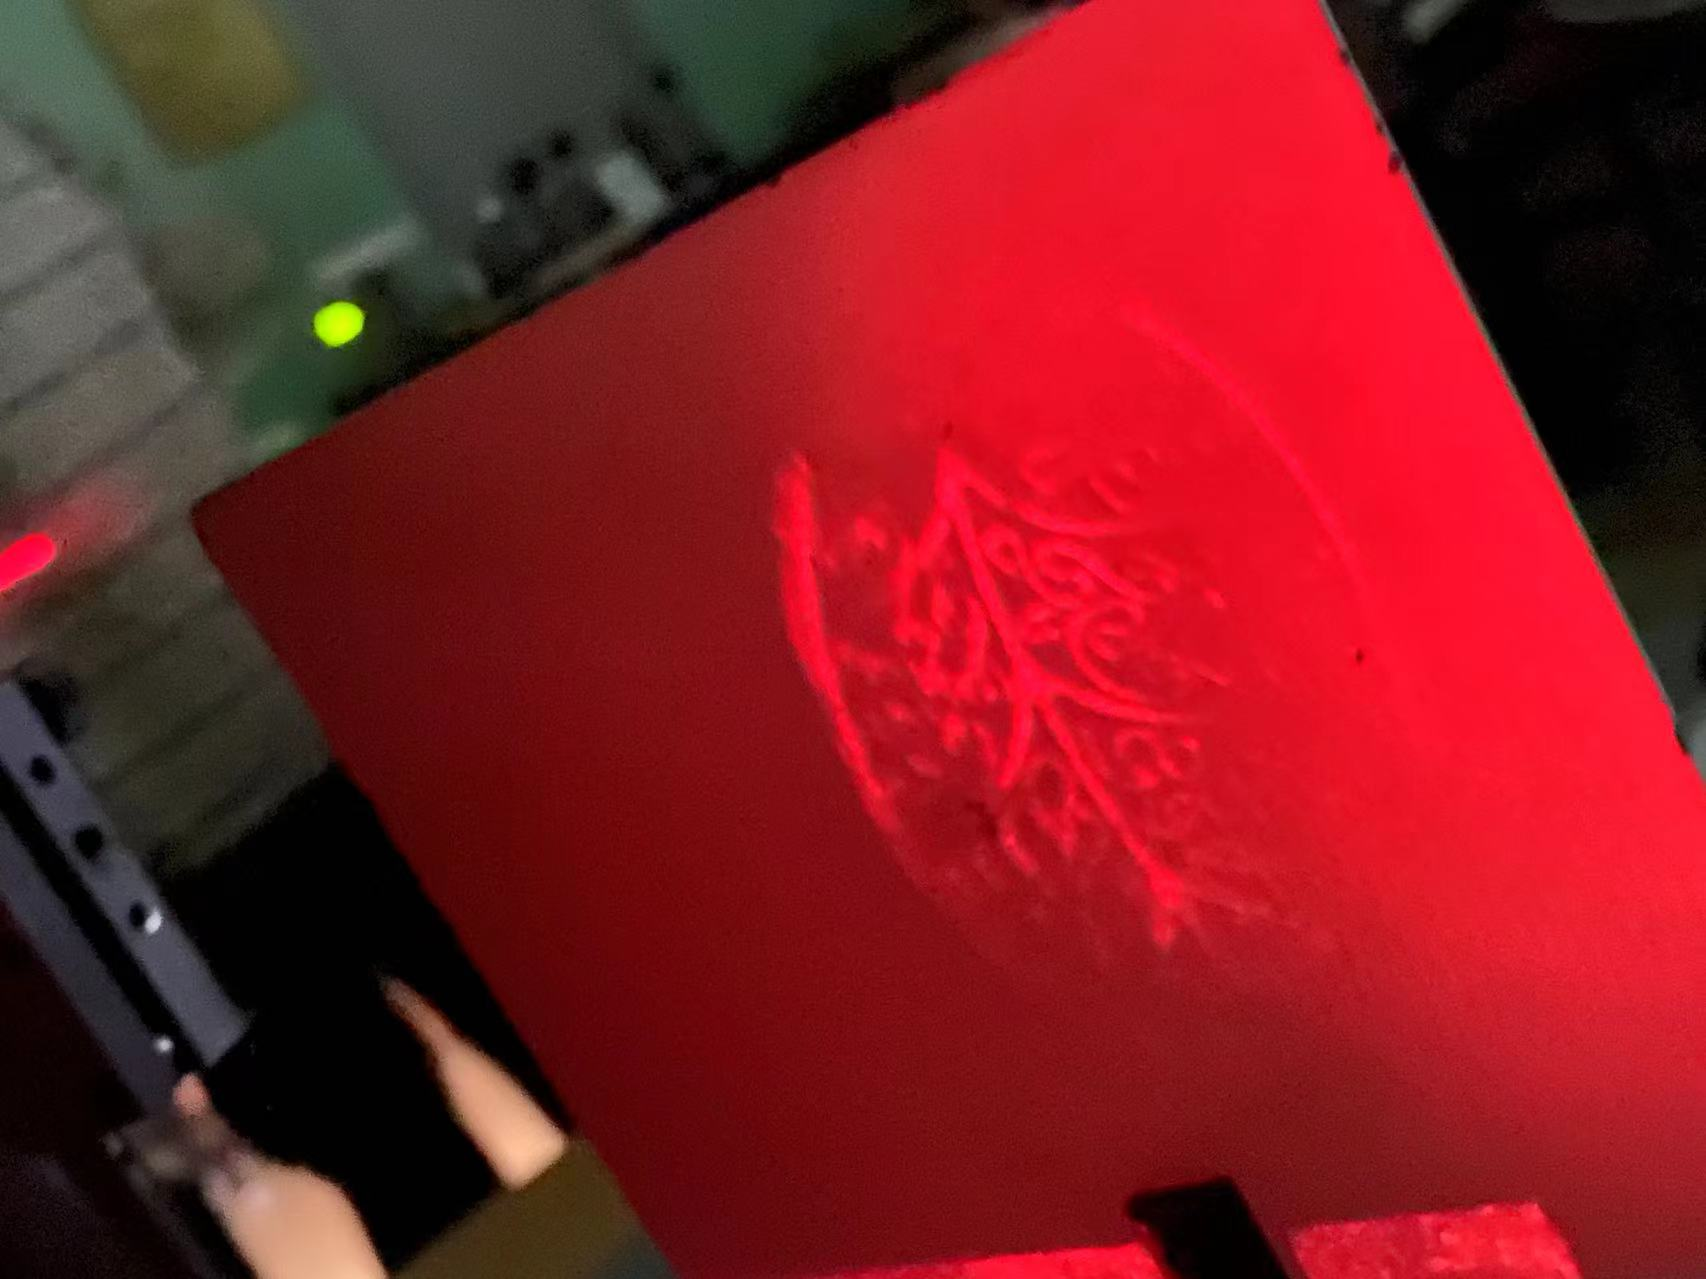
\includegraphics[width=.4\textwidth]{fig5.jpg}
    \caption{反转后再现的像}
\end{figure}

\subsection{利用激光直接照射重现观察}
\hspace{2em} 在本次实验中,使用肉眼可以观察到一个模糊的实像,光屏也存在一个实像,在本次实验观察到肉眼的距离是$\SI{157.6}{\cm}$,到底片的距离是$\SI{127.6}{\cm}$。\par
\hspace{2em} 分析:利用激光器直接照射,相当于一个平行光 \par
$$R^\prime=A$$
\hspace{2em} 由于记录时的参考光是一个发散球面光,其中的二次相因子作用相当于一个透镜,在透镜的作用下生成了一个实像。在本次实验由于使用的激光光强比使用的汇聚球面光要强,所以成的像更容易被观察到。\par
%%%%%%%%%%%%%%%%%%%%%%%%%%%%%%%%%%%%%%%%%%%%%%%%%%%%%%%%%%%%%%%%%%%

\subsection{感想}
\hspace{2em}在本次实验,除了动手验证了当时在光学课上学到的全息术以外,还接触到了暗室成像技术。加深了对相关知识的理解,同时开阔了知识面。感谢杨景老师的指导,并检查了实验中的数据。
\par

\end{document}